\documentclass[tikz,border=8pt]{standalone}
\usetikzlibrary{arrows.meta,calc}
\begin{document}
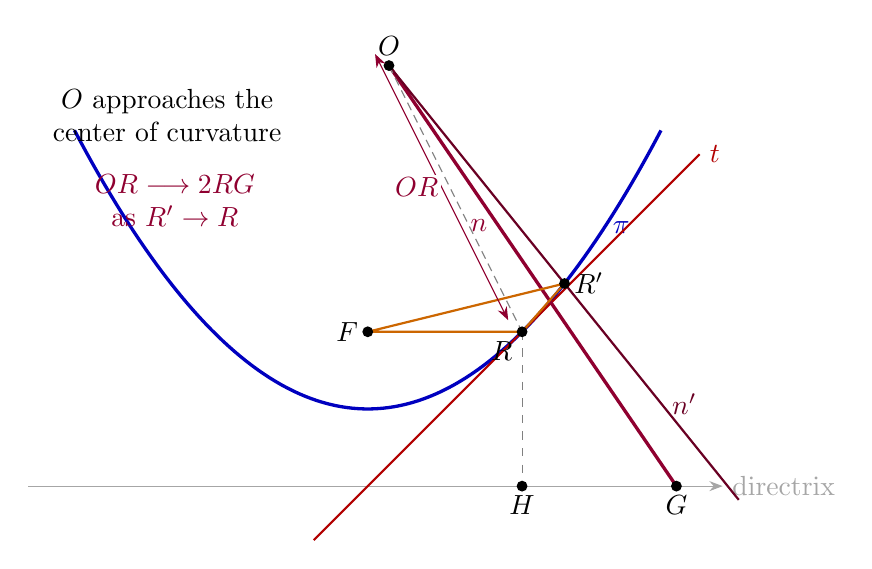
\begin{tikzpicture}[>=Stealth,scale=0.98]
  \draw[->,gray!70] (-4.4,0) -- (4.6,0) node[right] {directrix};
  \draw[blue!75!black,very thick,domain=-3.8:3.8,samples=100]
    plot (\x,{1 + (\x*\x)/4});
  \node[blue!75!black,right] at (3.05,3.35) {$\pi$};

  % R=(2,2), R'=(2.55,2.6256).  Their normals meet near O=(0.275,5.45).
  \coordinate (F) at (0,2);
  \coordinate (R) at (2,2);
  \coordinate (Rp) at (2.55,2.6256);
  \coordinate (H) at (2,0);
  \coordinate (G) at (4,0);
  \coordinate (O) at (0.275,5.45);

  \draw[red!70!black,thick] (-0.7,-0.7) -- (4.3,4.3) node[right] {$t$};
  \draw[purple!75!black,very thick] (G) -- (O) node[pos=.62,left] {$n$};
  \draw[purple!55!black,thick] ($(Rp)!-3.6cm!(O)$) -- (O) node[pos=.22,right] {$n'$};
  \draw[orange!80!black,thick] (F) -- (R) -- (Rp) -- (F);
  \draw[dashed,gray] (R) -- (H);
  \draw[densely dashed,gray] (O) -- (R);

  \fill (F) circle (2pt) node[left] {$F$};
  \fill (R) circle (2pt) node[below left] {$R$};
  \fill (Rp) circle (2pt) node[right] {$R'$};
  \fill (H) circle (2pt) node[below] {$H$};
  \fill (G) circle (2pt) node[below] {$G$};
  \fill (O) circle (2pt) node[above] {$O$};

  \draw[<->,purple!75!black] ($(R)+(-0.18,0.15)$) -- ($(O)+(-0.18,0.15)$)
    node[midway,left,fill=white,inner sep=1pt] {$OR$};
  \node[align=center] at (-2.6,4.8) {$O$ approaches the\\center of curvature};
  \node[align=center,purple!75!black] at (-2.5,3.7) {$OR\longrightarrow 2RG$\\as $R'\to R$};
\end{tikzpicture}
\end{document}
